%=====================================================================
\section{Lecture 10: Quantum sensing: which protocol measures which kernel}
\label{sec:lec10}

A qubit sensor is a two-level system whose coupling to the quantity of interest is exactly \cref{eq:model}: the ``signal'' is a classical or quantum field $B$, the ``noise'' is its fluctuating part, and the sensor's decoherence is the measurement.
The formalism of the previous lectures tells us precisely what is measured.
This lecture collects the results, with references to the sensing literature~\cite{Degen2017}, and ends with the one place where non-Markovian memory changes the metrological scaling.

\subsection{Relaxometry: the transverse sensor measures \texorpdfstring{$C(\pm\omega_0)$}{C(+-omega0)}}

For $\theta=\pi/2$ (or the transverse component of a general coupling) the population dynamics is governed by the two golden-rule rates of \cref{eq:rates-T1},
\begin{equation}
  \Gamma_\downarrow=C(\omega_0),\qquad \Gamma_\uparrow=C(-\omega_0),\qquad
  \Gamma_1=\Gamma_\downarrow+\Gamma_\uparrow=2S(\omega_0),\qquad
  \Gamma_\downarrow-\Gamma_\uparrow=2\chi''(\omega_0),
\end{equation}
(for $\sin\theta=1$).
Measuring the decay rate of the population \emph{and} its steady-state value therefore gives \emph{both} bath kernels at the qubit frequency: the noise $S(\omega_0)$ from $\Gamma_1$ and the response $\chi''(\omega_0)$ from the polarization $r_z^{\rm eq}=-\chi''(\omega_0)/S(\omega_0)$.
In a thermal bath the ratio is $\tanh(\beta\omega_0/2)$ and the qubit is a thermometer; in a driven or nonthermal environment the ratio defines an effective temperature at $\omega_0$, and the asymmetry $C(\omega_0)\ne C(-\omega_0)$ is the hallmark of \emph{quantum} noise, as emphasized by Schoelkopf \emph{et al.}~\cite{SchoelkopfClerk2003} and reviewed in~\cite[Sec.~II.B]{ClerkRMP2010}.
Sweeping $\omega_0$ (by a magnetic field, a flux, a gate voltage) maps $J(\omega)$: this is $T_1$ relaxometry.
In Keldysh language, $\Gamma_1$ comes from the $\qu\qu$ (Keldysh) component of the bath and $\Gamma_\downarrow-\Gamma_\uparrow$ from the $\qu\cl$ (retarded) component; the first column of \cref{eq:K2-bloch} says this directly.

At finite times the rates are the running integrals \eqref{eq:running-rates}.
Written in frequency space,
\begin{equation}
  \Gamma_\downarrow(t)=\sin^2\theta\int_{-\infty}^\infty\!\frac{\dd\omega}{\pi}\,C(\omega)\,\frac{\sin[(\omega-\omega_0)t]}{\omega-\omega_0},
  \label{eq:kofman}
\end{equation}
the bath spectrum is sampled through a filter of width $1/t$ around $\omega_0$.
Modulating the qubit (frequency sweeps, pulses) reshapes the filter: this is the Kofman--Kurizki universal formula for controlled decay~\cite{Kofman2000,Kofman2001}, and the Zeno and anti-Zeno effects are its short-time consequences.

\subsection{Dephasing: the longitudinal sensor measures \texorpdfstring{$S(\omega)$}{S(omega)} through a filter}

For $\theta=0$ the coherence is given exactly by \cref{eq:dephasing-exact}, $\rho_{01}(t)=\rho_{01}(0)\ee^{-i\omega_0t-\Gamma(t)}$.
A pulse sequence of $\pi$-pulses at times $t_1<t_2<\dots$ multiplies the integrand by the sign function $y(s)=\pm1$ that flips at each pulse, and the exponent becomes
\begin{equation}
  \boxed{\;\Gamma(t)=\frac4\pi\int_0^\infty\!\dd\omega\,\frac{S(\omega)}{\omega^2}\,F(\omega,t),\qquad
  F(\omega,t)=\frac{\omega^2}{2}\Big|\int_0^t\!\dd s\,y(s)\,\ee^{i\omega s}\Big|^2 ,\;}
  \label{eq:filter}
\end{equation}
with $F=1-\cos\omega t$ for free induction (Ramsey~\cite{Ramsey1950}), $F=8\sin^4(\omega t/4)$ for the Hahn echo~\cite{Hahn1950}, and comb-like filters for Carr--Purcell--Meiboom--Gill (CPMG)~\cite{CarrPurcell1954,MeiboomGill1958} and Uhrig sequences~\cite{Uhrig2007}; the general formalism is due to Cywi\'nski \emph{et al.}~\cite{Cywinski2008} (for Leggett's coupling normalization replace $4/\pi\to1/\pi$; normalizations of $F$ differ between papers).
Three statements follow from the structure of the formula.
\begin{itemize}[itemsep=1pt]
\item Only the \emph{noise} kernel enters.
  A pure-dephasing sensor is blind to $\chi$: every response line in the diagrams ends on an $S^\cl$, which annihilates the coherence (Example~4.3).
  It therefore cannot distinguish a quantum bath from a classical Gaussian noise with the same $S(\omega)$, and it cannot measure the temperature of the bath except through the $\coth$ in $S$.
\item The filter is set by the control, the spectrum by the bath.
  With $n$ equally spaced pulses (CPMG, spacing $\tau=t/n$) the filter approaches a comb at $\omega_k=k\pi/\tau$, $k$ odd, and
  \begin{equation}
    \Gamma(t)\simeq\frac{16\,t}{\pi^2}\sum_{k\ \mathrm{odd}}\frac{S(k\pi/\tau)}{k^2}\qquad(n\gg1),
    \label{eq:comb}
  \end{equation}
so that the decay rate measured as a function of $\tau$ is $S(\pi/\tau)$ up to harmonics.
This is noise spectroscopy by dynamical decoupling~\cite{AlvarezSuter2011,Yuge2011}, realized e.g.\ in~\cite{Bylander2011}; the general transfer-function viewpoint is in~\cite{Paz2017}.
\item The exponent is a quadratic functional of $y$: this is the statement that the influence functional \eqref{eq:FV} is quadratic in $s^\qu$ for a Gaussian bath.
  For a non-Gaussian bath, higher cumulants add terms of higher order in $y$, and the decoupling sequences no longer act as linear filters.
\end{itemize}

\begin{figure}[t]
\centering
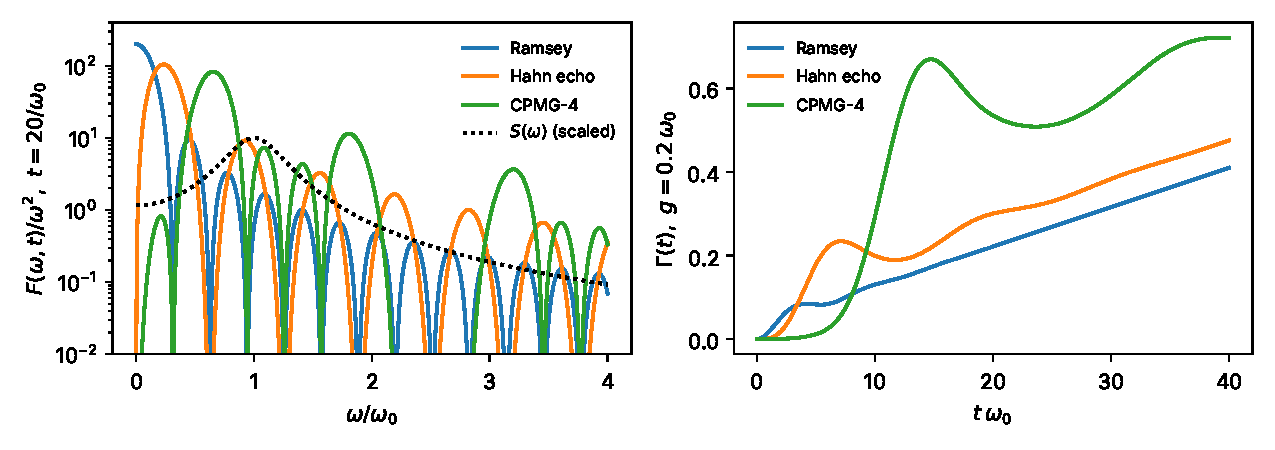
\includegraphics[width=\textwidth]{figures/fig_filter.pdf}
\caption{Left: filter functions $F(\omega,t)/\omega^2$ at $t=20/\omega_0$ for free induction, Hahn echo and CPMG with four pulses, against the Lorentzian noise spectrum of the running example.
Right: the resulting $\Gamma(t)$ (computed for the coupling $\tfrac12\sz\otimes B$, i.e.\ with $1/\pi$ in \cref{eq:filter}) at $g=0.2\omega_0$.
The CPMG curve shows a bump near $t\omega_0\approx4\pi$, where the comb's first tooth $\pi/\tau=4\pi/t$ sweeps through the bath resonance at $\Omega=\omega_0$: the sequence has detected the spectral line.}
\label{fig:filter}
\end{figure}

\subsection{The mixed sensor}

For general $\theta$ both channels are open.
In the secular (weak-coupling, long-time) regime the Ramsey signal decays at $\Gamma_2=\tfrac12\Gamma_1+\Gamma_\varphi$ with $\Gamma_1\propto\sin^2\theta\,S(\omega_0)$ and $\Gamma_\varphi\propto\cos^2\theta\,S(0)$, so a Ramsey measurement alone cannot separate low-frequency from resonant noise; a $T_1$ measurement is needed to subtract the $\Gamma_1/2$ part.
Dynamical decoupling filters only the $\cos^2\theta$ part: $\pi$-pulses about $\hat x$ commute with $\sx$, so the transverse coupling is not refocused, and the echo decay saturates at $\ee^{-\Gamma_1t/2}$.
Outside the secular regime the cross terms $\cos\theta\sin\theta$ of \cref{eq:K2-bloch} mix populations and coherences, and the pseudomode numerics of \cref{fig:dynamics} is the honest way to design a protocol.

\subsection{Precision scaling: when memory matters}

Frequency estimation by Ramsey interferometry with $N$ qubits and total time $T$: each run of duration $t$ yields a signal $\tfrac12[1+\ee^{-\Gamma(t)}\cos\omega_0t]$, with Fisher information $t^2\ee^{-2\Gamma(t)}$ per qubit per run at the optimal phase~\cite{Braunstein1994}.
With $T/t$ runs the Cram\'er--Rao bound reads
\begin{equation}
  \delta\omega_0^2\ \ge\ \frac{1}{N\,T\,t\,\ee^{-2\Gamma(t)}}\qquad\text{(product state)},\qquad
  \delta\omega_0^2\ \ge\ \frac{1}{N^2\,T\,t\,\ee^{-2N\Gamma(t)}}\qquad\text{(GHZ state)},
\end{equation}
the Greenberger--Horne--Zeilinger (GHZ) state~\cite{GHZ1989} acquiring the phase $N\omega_0t$ but, for independent baths, also $N$ times the dephasing exponent.
Optimizing over $t$:
\begin{center}
\renewcommand{\arraystretch}{1.3}
\begin{tabular}{@{}lll@{}}
\toprule
& product state & GHZ state\\
\midrule
Markov, $\Gamma=\gamma t$ & $t^*=\tfrac1{2\gamma}$, $\ \delta\omega_0^2=\dfrac{2e\gamma}{NT}$ & $t^*=\tfrac{1}{2N\gamma}$, $\ \delta\omega_0^2=\dfrac{2e\gamma}{NT}$ (no gain)\\[6pt]
Zeno regime, $\Gamma=\kappa t^2$ & $t^*=\tfrac{1}{2\sqrt\kappa}$, $\ \delta\omega_0^2=\dfrac{2\sqrt{e\kappa}}{NT}$ & $t^*=\tfrac{1}{2\sqrt{N\kappa}}$, $\ \delta\omega_0^2=\dfrac{2\sqrt{e\kappa}}{N^{3/2}T}$\\
\bottomrule
\end{tabular}
\end{center}
The first row is the classic result that Markovian dephasing erases the quantum advantage of entanglement~\cite{Huelga1997}.
The second row is the observation of Matsuzaki, Benjamin and Fitzsimons~\cite{Matsuzaki2011} and of Chin, Huelga and Plenio~\cite{Chin2012}: when the optimal interrogation time falls inside the initial quadratic (Zeno) regime of $\Gamma(t)$, which it does for a GHZ state at large $N$ because $t^*\propto N^{-1/2}$, the precision scales as $N^{-3/4}$, between the standard quantum limit $N^{-1/2}$ and the Heisenberg limit $N^{-1}$.
In the language of these notes: the short-time behaviour $\Gamma(t)\simeq2g^2t^2\cdot(\ldots)$ follows from $K(0)=K^{(2)}(0)\ne0$ (\cref{sec:nz-irreducible}): a memory kernel that is finite at $\tau=0$ always produces a quadratic onset, and the crossover time to linear decay is the bath correlation time $\tau_B$.
The Markov row applies when $t^*\gg\tau_B$, the Zeno row when $t^*\ll\tau_B$.
The numbers in \cref{eq:lorentz-kernels} give $\kappa=2g^2\cos^2\theta+g^2\sin^2\theta$ (dephasing plus half of the transverse channel) and $\tau_B=2/\gamma$ for the Lorentzian bath.

\subsection{Which formalism for which question}

\begin{center}
\small
\renewcommand{\arraystretch}{1.25}
\begin{tabularx}{\textwidth}{>{\raggedright\arraybackslash}p{4.2cm}>{\raggedright\arraybackslash}X}
\toprule
\textbf{Question} & \textbf{Natural tool}\\
\midrule
Which bath quantity does protocol X measure? & Keldysh rotation: $\qu\qu$ lines $\to S$, $\qu\cl$ lines $\to\chi$; read off from the diagram (\cref{sec:lec4}).\\
Exact dephasing under arbitrary control & Influence functional with c-number $y(s)$ (\cref{sec:lec7}); filter functions.\\
Rates, steady state, thermometry & Second-order NZ/TCL, secular limit (\cref{sec:lec5}); FDT fixes $\chi''/S$.\\
Short-time (Zeno) behaviour, precision scaling & TCL2 running rates (\cref{sec:lec6}); $K(0)\neq0$.\\
Strong coupling, incoherent regime & Polaron frame, NIBA and beyond (\cref{sec:lec7}).\\
Linear response of the sensor to a drive & Mori / retarded self-energy (\cref{sec:lec8}).\\
Back-action on the bath (a cavity, a line) & Keldysh Dyson equation for the dressed bath propagator (\cref{sec:lec9}).\\
Benchmarking any of the above & Pseudomode exact solution (\cref{sec:lec2,sec:numerics}).\\
\bottomrule
\end{tabularx}
\end{center}

\subsection{Exercises}

\begin{exercise}\label{ex:10-1}
Derive \cref{eq:kofman} from the running rate $\Gamma_\downarrow(t)=2\sin^2\theta\,\Re\int_0^t\ee^{i\omega_0\tau}C(\tau)\dd\tau$ and show that a periodic modulation of $\omega_0$ shifts the filter.
Explain the anti-Zeno effect for a bath whose $C(\omega)$ rises above $\omega_0$.
\end{exercise}

\begin{exercise}\label{ex:10-2}
Derive the Hahn-echo filter $F=8\sin^4(\omega t/4)$ and \cref{eq:comb}.
Use the Lorentzian $S(\omega)$ to reproduce the bump in \cref{fig:filter} analytically: at what $t$ does it appear for CPMG with $n$ pulses?
\end{exercise}

\begin{exercise}\label{ex:10-3}
Repeat the Fisher-information analysis for $T_1$-limited sensing (a transverse sensor) and for a Ramsey sensor with $\Gamma(t)=\Gamma_2t+\kappa t^2$.
Where is the crossover between the two rows of the table, in terms of $\tau_B$ and $N$?
\end{exercise}

\begin{exercise}\label{ex:10-4}
(Capstone.)
For the Lorentzian bath with $\theta=\pi/4$, use the pseudomode script to simulate a Hahn echo (insert a $\pi$-pulse about $\hat x$ at $t/2$) and compare the echo amplitude with (a) the filter-function prediction using only the $\cos^2\theta$ part and (b) the same multiplied by $\ee^{-\Gamma_1t/2}$.
Discuss the residual discrepancy in terms of the $\cos\theta\sin\theta$ terms of \cref{eq:K2-bloch}.
\end{exercise}

\clearpage
